 \documentclass[a4paper,12pt]{article}
\usepackage[a4paper,top=3cm,bottom=2cm,left=3cm,right=3cm,marginparwidth=1.75cm]{geometry}
\usepackage[brazil]{babel}
\usepackage[T1]{fontenc}
\usepackage[utf8]{inputenc}
\usepackage{amsmath}
\usepackage{MnSymbol}
\usepackage{wasysym}
\usepackage{hyperref}
\usepackage{color}
\definecolor{Blue}{rgb}{0,0,0.9}
\definecolor{Red}{rgb}{0.9,0,0}
\usepackage{esvect}
\usepackage{graphicx}
\usepackage{float}
\usepackage{indentfirst}
\usepackage{caption}
\usepackage{blkarray}
\newcommand\Mark[1]{\textsuperscript#1}
\usepackage{pgfplots}
\usepackage{amsfonts}
\usepackage[english, ruled, linesnumbered]{algorithm2e}
\usepackage{algorithmic}
%\usepackage[toc,page]{appendix}
\newtheorem{definicao}{Definição}[section]
\newtheorem{teorema}{Teorema}[section]

\title{Geometria de Distâncias}
\author{Guilherme Philippi}
\begin{document}
\maketitle
\tableofcontents

\section{Geometria de Distâncias Euclidianas}
Apresenta-se nesta seção uma introdução a \textit{Geometria de Distâncias Euclidianas}. O nome ``Geometria de Distâncias'' diz respeito ao conceito desta geometria basear-se em distâncias ao invés de pontos. A palavra ``Euclidiana'' é importante para caracterizar as arestas --- elementos fundamentais associados as distâncias --- como segmentos, sem restringir seus ângulos de incidência \cite{libertiEDG}.

\subsection{Como tudo Começou}

Por volta de 300 AC, Euclides de Alexandria organizou o conhecimento de sua época acerca da Geometria em uma obra composta por treze volumes, onde construiu, a partir de um pequeno conjunto de axiomas fortemente baseado nos conceitos de pontos e linhas, a chamada \textit{Geometria Euclidiana} \cite{elementosEuclides}. Em contraponto a visão original de Euclides, os primeiros conceitos geométricos usando \textit{apenas distâncias} costumam estar associados aos trabalhos de Heron de Alexandria (10 a 80 DC) \cite{libertiEDG}, com o desenvolvimento de um teorema que leva seu nome, como segue: 
\begin{center}
	\begin{minipage}{0.9 \linewidth}
		\textbf{\textit{Teorema de Heron}:} Sejam $s$ o \textit{semiperímetro} de um triângulo (se $p$ é o perímetro, $s = \frac{p}{2}$) e $a$, $b$ e $c$ os comprimentos dos três lados deste triangulo. Então, a área $A$ do triângulo é
		
		\begin{equation}\tag{Fórmula de Heron}
		A = \sqrt{s(s-a)(s-b)(s-c)}.
		\label{eq:heron}
		\end{equation}
	\end{minipage}
\end{center} 
Pode-se dizer que esse foi o nascimento da \textit{Geometria de Distâncias} (\textit{Distance Geometry}, ou DG).

Algumas centenas de anos depois, em 1841, Arthur Cayley (1821 a 1895) generalizou a~\ref{eq:heron} através da construção de um determinante que calcula o conteúdo (volume $n$-dimensional) de um \textit{simplex}\footnote{Um simplex é uma generalização do conceito de triangulo a outras dimensões, i.e.: O \textit{0-simples} é um ponto, \textit{1-simplex} é um segmento de reta, \textit{2-simplex} é um triangulo e o \textit{3-simplex} é um tetraedro.} em qualquer dimensão \cite{cayley1841HaronGD}. Um século depois, em 1928, o matemático austríaco Karl Menger (1902 a 1985) re-organizou as ideias de Cayley e trabalhou em uma construção axiomática da geometria através de distâncias \cite{mengerDeterminante} --- donde a alteração no nome do determinante de Cayley para como é conhecido hoje: ``\textit{Determinante de Cayley-Menger}''.  

\begin{center}
	\begin{minipage}{0.9 \linewidth}
		\textbf{Definição:} Sejam $A_0, A_1, \dots, A_n$ $n + 1$ pontos que definem os vértices de um $n$-simplex em um espaço euclidiano $K$-dimensional, onde $n\leq K$, e seja $d_{ij}$ a distância entre os vértices $A_i$ e $A_j$, onde $0\leq i < j \leq n$. Então, o conteúdo $v_n$ desse $n$-simplex é
	\end{minipage}
\end{center} 

\vspace{-0.5cm}

\begin{equation}\tag{Determinante de Cayley-Menger}
v_n^2 = \frac{(-1)^{n+1}}{(n!)^22^n}
\begin{vmatrix}
0 & d^2_{01} &  d^2_{02} & \ldots & d^2_{0n} & 1\\ 
d^2_{01} & 0 & d^2_{12} & \ldots & d^2_{1n} & 1\\ 
d^2_{02} & d^2_{12} &  0 & \ldots & d^2_{2n} & 1\\ 
\vdots & \vdots &  \vdots & \ddots & \vdots & \vdots\\ 
d^2_{0n} & d^2_{1n} & d^2_{2n}  & \ldots & 0 & 1\\ 
1 & 1 & 1  & \ldots & 1 & 0\\ 
\end{vmatrix}.
\label{determinanteCayleyMenger}
\end{equation}

Mas foi só com Leonard Blumenthal (1901 a 1984) que, em 1953, o termo Geometria de Distâncias foi cunhado --- com a publicação de seu livro \textit{``Theory and Applications of Distance Geometry''} \cite{Blumenthal:53}.
Blumenthal dedicou sua vida de trabalho para clarificar, organizar e traduzir as obras originais em alemão \cite{libertiEDG}. Ele acreditava que o problema mais importante nesta área era o \textit{``Problema de Subconjunto''} (ou \textit{Subset Problem}, originalmente), que consistia em encontrar condições necessárias e suficientes a fim de decidir quando uma matriz simétrica era, de fato, uma \textit{matriz de distâncias}\footnote{Seja o par $(\mathcal{X}, d)$ um \textit{espaço métrico} (vide Apêndice~\ref{ap:metric}), onde $\mathcal{X} = \{x_1, \dots, x_n\}$. Uma \textit{matriz de distância sobre $\mathcal{X}$} é uma matriz quadrada $D_{n\times n} = (d_{uv})$ onde, para todo $u,v \leq n$, temos $d_{uv} = d(x_u,x_v)$ \cite{carlileGDandAplications}.} \cite{carlileGDandAplications}. Uma restrição desse problema à métrica euclidiana chama-se \textit{Problema de Matrizes de Distâncias Euclidianas} (ou EDMP, do inglês \textit{Euclidean Distance Matrix Problem}), como segue definida:

\begin{center}
	\begin{minipage}{0.9 \linewidth}
		\label{EDMP}
		\textbf{Problema de Matrizes de Distâncias Euclidianas:} Determinar se, para uma dada matriz quadrada $D_{n\times n} = (d_{ij})$, existe um inteiro $K$ e um conjunto $\{p_1, \dots, p_n \}$ de pontos em $\mathbb{R}^K$ tal que $d_{ij} = \lVert p_i - p_j\rVert$ para todo $i,j \leq n$.
	\end{minipage}
\end{center} 

Condições necessárias e suficientes para que uma matriz seja, de fato, uma matriz de distância euclidiana são dados em \cite{EDMPResolucao}. Para isso, apresenta-se um teorema onde se utiliza o~\ref{determinanteCayleyMenger} na criação de duas condições afirmando que, afim de $D_{n\times n}$ ser uma matriz de distâncias euclidianas, deve haver um $K$-simplex $S$ de referência com conteúdo $v_K \neq 0$ em $\mathbb{R}^K$ e que todos os $(K+1)$-simplex e $(K+2)$-simplex contendo S como uma das faces devem estar contidos em $\mathbb{R}^K$ \cite{carlileGDandAplications}.

Blumenthal percebeu a importância em se respeitar as restrições métricas estabelecidas pelas matrizes de distâncias.
\begin{quotation}
	\textit{Quando temos como dado um conjunto de distâncias entre pares de pontos, a geometria das distâncias pode dar uma dica para encontrar um conjunto de coordenadas correto para pontos no espaço Euclideano tridimensional, satisfazendo as restrições de distâncias dadas.}
	\begin{flushright}
		(Blumenthal, 1953, \cite{Blumenthal:53})
	\end{flushright}
\end{quotation}

Pode-se dizer que resolver o Problema de Matrizes de Distâncias Euclidianas está intimamente relacionado com descobrir as coordenadas dos pontos que definem suas distâncias. Perceba que este é um problema inverso, onde o ``problema direto'' correspondente é calcular distâncias associadas a pares de pontos dados. Note que este estudo tem enorme aplicabilidade \cite{carlileGDandAplications}.
\\

Adiante, em 1979, Yemini (atualmente professor emérito de Ciência da Computação na Universidade de Columbia) foi o primeiro a flexibilizar a definição do EDMP ao considerar um conjunto de distâncias esparso \cite{Yemini:79,carlileGDandAplications} --- i.e., que não se tem todas as distâncias dadas a priori. Com isso, introduziu-se o que se chamou de \textit{Problema Posição - Localização}, onde deseja-se calcular a localização de todos os objetos imersos em um espaço geográfico \cite{Yemini:79}. 

Assim, foi possível re-formular o problema fundamental de Geometria de Distâncias, o qual pode ser caracterizado de forma mais moderna pela utilização da Teoria de Grafos \cite{carlileGDandAplications}.

\subsection{O Problema Fundamental}

Uma \textit{realização} é uma função que mapeia um conjunto de vértices de um grafo $G$ para um espaço euclidiano de alguma dimensão dada \cite{libertiEDG}.

\begin{center}
	\begin{minipage}{0.9 \linewidth}
		\textbf{Problema de Geometria de Distâncias (DGP):} Dados um grafo simples, ponderado e conectado $G = (V, E, d)$ e um inteiro $K>0$, encontre uma realização $x: V \longrightarrow \mathbb{R}^K$ tal que:
		\begin{equation}
		\forall \{u,v\} \in E, \hspace{0.5cm} \lVert x(u) - x(v) \rVert = d(u,v). \label{eq:DGP}
		\end{equation}
	\end{minipage}
\end{center}

Desde que uma realização seja encontrada, também dá-se a ela o nome de \textit{solução} do DGP. Por simplicidade --- claramente um abuso de notação ---, pode-se escrever $x_u$ e $d_{uv}$ no lugar de $x(u)$ e $d(u,v)$, respectivamente.

A principal diferença desta definição para o EDMP está acerca de que uma matriz de distância essencialmente representa um \textit{grafo ponderado completo}. Em contraponto, o DGP não empoe qualquer estrutura em $G$\footnote{A menos, é claro, no que diz respeito a seus vértices estarem conectados. Porém, caso $G$ não seja conectado, então ele consiste de um conjunto de diferentes subgrafos conectados, donde, a fim de solucionar o DGP, pode-se realizar cada subgrafo separadamente \cite{libertiEDG}.}, seguindo o conceito de matriz esparsa estabelecido por Yemini.

Por fim, na equação~\ref{eq:DGP}, utiliza-se a norma euclidiana $\lVert$ $\cdot$ $\rVert$ como métrica (ver Apêndice~\ref{ap:metric}), donde pode-se reescrever esta equação como

\begin{equation*}
	\forall \{u,v\} \in E, \hspace{0.5cm} \sqrt{\sum_{i=1}^{K}(x_{ui} - x_{vi})^2} = d_{uv}.
\end{equation*}

Como a definição de métrica garante a positividade das distâncias, pode-se esconder a raiz quadrada na equação acima, i.e.

\begin{equation}
\forall \{u,v\} \in E, \hspace{0.5cm} \sum_{i=1}^{K}(x_{ui} - x_{vi})^2 = d_{uv}^2.
\label{eq:DGPSistemaQuadratico}
\end{equation}

\subsection{Os Diferentes Problemas em DG}

Em 2014, Leo Liberti \textit{et al.} publicaram um ótimo compendio sobre a \textit{Geometria de Distâncias Euclidianas e suas Aplicações} \cite{carlileGDandAplications} e, em particular, desenvolveram um estudo  taxonômico muito interessante sobre os problemas clássicos da área. No que se segue, devido a grande quantidade de siglas e variações dentro de DG, apresenta-se parte desse estudo, visando organizar os conceitos. 
\\

As principais aplicações em DG são no \textit{calculo de estruturas moleculares} \cite{crippen:DistancesAndMolecularConformation}, na \textit{localização de sensores em rede sem fio} (\textit{Wireless Sensor Network Localization}, ou WSNL) \cite{yemini1978positioning}, em \textit{cinemática inversa} (\textit{Inverse Kinematic}, ou IK) \cite{cinematicaInversa} e em \textit{escalonamento multidimensional} (\textit{Multidimensional Scaling}, ou MDS) \cite{multidimensionalScaling}.

\subsubsection{Conformações Moleculares}

Existe uma relação muito forte com a forma geométrica das moléculas e suas funções em organismos vivos \cite{bioquimicaLehninger}. Projetar drogas para curar uma doença específica se trata basicamente de conhecer o que uma certa proteína pode fazer em um organismo \cite{libertiEDG}. Proteínas se ligam em outras moléculas através do equilíbrio de forças agindo entre elas\footnote{Ou seja, o equilíbrio da energia potencial das moléculas, proporcional, principalmente, as variações nos comprimentos das ligações covalentes, as variações nos ângulos entre duas ligações covalentes consecutivas, as rotações sobre as ligações covalentes e as interações de van der Waals e interações eletrostáticas entre átomos \cite{carlileTese}.}, por tanto, suas ligações dependem do seu formato. 

Proteínas são constituídas por um grande conjunto de átomos e, alguns pares destes, trocam ligações químicas --- sabe-se quais são esses átomos através de experimentos de cristalografia \cite{ramachandran1974MolStructure}. Então, se os átomos de uma molécula forem rotulados da forma $1,3,4,\dots,n$, então é possível inferir: 
\begin{itemize}
	\item O conjunto de ligações $\{u,v\}$, onde $u,v$ são átomos em $\{1,\dots,n\}$;
	\item A distância entre $u$ e $v$ (para cara par ligado);
	\item O ângulo interno $\theta_v$ definido por duas ligações $\{u,v\}$ e $\{v,w\}$, com um átomo $v$ em comum. (veja o Apêndice~\ref{ap:cos})
\end{itemize} 

Além desses dados, também é possível obter informações a partir de experimentos mais sofisticados, como a \textit{Ressonância Magnética Nuclear} (RMN). Neste experimento é escolhida uma faixa de radiofrequência para bombardear uma amostra que está imersa em um campo magnético bastante intenso. Dependendo da radiofrequência utilizada (costuma-se usar a do hidrogênio), alguns núcleos atômicos irão absorver energia e outros não. Caso atinja-se uma frequência exata de ressonância dentro destes núcleos atômicos, é possível medir essa ressonância como um sinal de radiofrequência enviado dos núcleos atômicos --- para calcular distâncias entre átomos próximos, com distâncias menores que 5\AA.

De posse dessas informações, deseja-se realizar (localizar) todos os átomos da molécula. Esse problema, com todas as informações moleculares disponíveis, denomina-se \textit{Estrutura Proteica a partir de Dados Brutos} (\textit{Protein Structure from Raw Data}, ou PSRD)

Em particular, como as coordenadas atômicas pertencem ao $\mathbb{R}^3$, há uma particularização do DGP para o caso molecular, chamado \textit{Problema de Geometria de Distâncias Moleculares} (\textit{Molecular DGP}, ou MDGP). Trata-se do DGP com $K = 3$ fixo.

\subsubsection{Localização de Sensores}

O \textit{Problema de Localização de Sensores em Rede sem Fio} (ou \textit{WSNL Problem}) surge quando é necessário localizar um conjunto de objetos equipados com sensores eletrônicos capazes de medir distâncias entre si, geograficamente distribuídos, usando apenas medidas de distâncias entre pares destes objetos \cite{yemini1978positioning}. 

Por exemplo, \textit{smartphones} com WIFI ativo podem criar uma rede conhecida por \textit{Rede Ad-Hoc}, \textit{i.e.}, eles conseguem criar uma rede para comunicar-se entre si, de forma \textit{peer-to-peer}, sem a necessidade de uma torre central --- cada aparelho funciona como uma pequena torre, de forma que a distância entre os aparelhos não pode ser excessiva.
Dessa forma, os \textit{smartphones} podem estimar a distância $r$ de emparelhamento das suas conexões ao medir, por exemplo, qual a potência de transmissão do sinal, uma vez que sabe-se que a potência $P$ de uma transmissão eletromagnética cai da forma 
\begin{equation}
	P = \frac{X}{r^n},
\end{equation}
onde $X$ e $n$ são constantes e dependem muito das condições do experimento, sendo obtidas experimentalmente \cite{savvides2001dynamic}.

Em essência, um problema do tipo WSNL segue a mesma definição do DGP, porém, com um subconjunto $A\subset V$ de vértices (chamados \textit{âncoras}), onde os elementos de $A$ tem uma posição em $\mathbb{R}^k$ dada a priori --- isso é feito pois, normalmente, interessa saber a posição relativa de um objeto a outro, como é o caso do Sistema de Posicionamento Global, onde temos os satélites como âncoras e desejamos saber a posição dos aparelhos GPS em relação aos satélites.

Por motivos práticos --- semelhantes ao caso molecular --- as variações de interesse desse problema tem o $K$ fixo em $K= 2$ ou $K=3$.

\subsubsection{Dinâmicas em Cinemática Inversa}

Muito utilizada em robótica e animação computadorizada, a cinemática inversa cerne sobre mecanismos e seus movimentos rígidos, onde restringe-se os movimentos de forma a preservar a geometria do sistema. Sem o auxilio computacional e matemático a manipulação de mecanismos com muitos graus de liberdade  pode ser inviável: Imagine a manipulação manual de cem vértices em uma haste simulando o comportamento de um braço articulado em uma animação. Com o auxílio da DG, um animador pode apenas configurar a posição final de um pequeno grupo de vértices (como os da extremidade da aresta, por exemplo) e um algorítimo de cinemática inversa é capaz de verificar se aquela posição é ou não viável e, se viável, qual a realização de todo o conjunto de vértices em razão da posição configurada \cite{cinematicaInversa}.

Visando tal restrição mecânica, define-se o \textit{Problema de Cinemática Inversa} (\textit{Inverse Kinematic Problem}, ou IKP) como uma variação do WSNL --- logo, tem o objetivo de descobrir posições em relação a certos pontos previamente realizados --- com uma restrição no grafo que define o problema: deve ser um caminho simples com seus vértices finais sempre sendo âncoras \cite{carlileGDandAplications}.

\subsubsection{Escalonamento Multidimensional}

O problema de \textit{Escalonamento Multidimensional} (\textit{Multidimensional Scaling}, ou MDS)
é definido como \cite{carlileGDandAplications}: Dado um conjunto $X$ de vetores, encontre um conjunto $Y$ de vetores com menor dimensão (com $|X| = |Y|$) tal que a distância entre cada $i$-ésimo e $j$-ésimo vetores de $Y$ tenham, aproximadamente, a mesma distância que seus pares de vetores correspondentes em $X$.

Esse problema é muito aplicado na analise de dados em Big Data \cite{libertiEDG}. É um meio de facilitar a visualização do nível de similaridade entre casos individuais --- que não necessariamente precisam ter uma conexão aparente --- em um conjunto de dados. Pode-se usá-lo, por exemplo, para visualizar em uma escala bidimensional ($\mathbb{R}^2$) a evolução da locomoção de animais no espaço tridimensional utilizando dados de séries temporais (espaço em diferentes tempos, logo, dados em $\mathbb{R}^4$).

\subsection{A Busca de uma Solução}

A abordagem mais simples, pode-se pensar, para encontrar um conjunto de soluções que satisfação a equação~\ref{eq:DGPSistemaQuadratico} é resolver o sistema de equações diretamente \cite{carlileBook31Coloquio}. Infelizmente, para $K \geq 2$, há evidencias de que uma solução de forma fechada onde todo componente de $x$ é expresso por raízes, não é possível \cite{libertiEDG}. 

No entanto, pode-se re-formular o problema como um problema de otimização global \cite{libertiEDG}, onde o objetivo é minimizar a soma dos erros\footnote{Em otimização, vê-se a equação~\ref{eq:DGP} de forma não exata: $\lVert x_u - x_v \rVert = d_{uv} + \varepsilon$, onde $\varepsilon$ é chamado \textit{erro}. Ou seja, para minimizar o erro, precisa-se minimizar a expressão $f(x_u,x_v) = \lVert x_u - x_v \rVert - d_{uv}$.} entre as distâncias dadas a priori e as calculadas. Para isso, pode-se considerar uma única expressão que englobe todos os $n$ erros, da forma
\begin{equation}
	f(x_1,\dots,x_n) = \sum_{(i,j)\in E} \left(\lVert x_i - x_j \rVert - d_{ij}\right)^2.
\end{equation}

Fica claro que encontrar uma solução para o DGP é equivalente a encontrar realizações $x_i \in \mathbb{R}^3$, $i=1,\dots,n$, se e somente se $f(x_1,\dots,x_n) = 0$ \cite{libertiEDG}. Pela definição de métrica (vide Apêndice~\ref{ap:metric}), 0 é o menor valor possível para $f$, donde diz-se que deseja-se \textit{minimizar a função} $f: \mathbb{R}^n \longrightarrow \mathbb{R}$ \cite{carlileBook31Coloquio}. Ou seja,
\begin{equation}
	\min_{x_i \in \mathbb{R}^n} f(x_1,\dots,x_n).
\end{equation}

Donde, no caso da métrica euclidiana \cite{libertiEDG}, temos

\begin{equation}
 \min_{x_j \in \mathbb{R}^n} \sum_{(u,v)\in E} \left(\sum_{i=1}^{K}(x_{ui} - x_{vi})^2 - d_{uv}^2\right)^2
 \label{eq:DGPminEuclid}
\end{equation}

Por tanto, a equação~\ref{eq:DGPminEuclid} tem como objetivo a minimização de um polinômio de múltiplas variáveis de grau quatro. 
\\

Um dos desafios da Otimização Global é que muitos dos métodos existentes --- em especial, os mais eficientes --- não garantem que uma otimização global será encontrada \cite{libertiEDG}. Isso se dá pois, dependendo do comportamento da função que se deseja otimizar, existem muitos ótimos locais e os métodos não conseguem diferenciá-los de um global. Em DG, a distribuição geometria dos vértices do grafo está intimamente ligada com o comportamento da função objetivo --- donde, por exemplo, em WSNL, é interessante o estudo de como distribuir os sensores afim de otimizar a busca por ótimos globais \cite{eren2004rigidity}.

\subsection{A Quantidade de Soluções}
Pode-se verificar que, dada uma solução de um DGP, obtêm-se facilmente uma quantidade infinita (não enumerável!) de outras realizações válidas, distintas, através de rotações e translações desta solução inicial \cite{carlileBook31Coloquio} --- Para que não se tenha tais soluções redundantes, costuma-se fixar a realização dos três primeiros vértices.

\subsubsection{Realização de Grafos Completos}

Para DGP definido em um espaço de dimensão $K$, a classe de problemas mais simples de resolver são dos grafos $(K+1)$-cliques, isto é, dos grafos completos com $K+1$ vértices \cite{libertiEDG}.



Note que um $K$-simplex é uma realização de um $(K+1)$-clique em $\mathbb{R}^K$. No geral, 


\newpage
\phantomsection
\addcontentsline{toc}{section}{Referências}

\bibliographystyle{unsrt}
\bibliography{references}

\appendix
\newpage
\section{Métricas}
\label{ap:metric}

Como esse texto utiliza fortemente o conceito de distância, é necessário e bem vindo que se gaste algum espaço para uma construção formal dessa ideia. A noção de distância está relacionada com o conceito de \textit{métrica}, como segue.
\\

Seja $\mathcal{X}$ um espaço vetorial $K$-dimensional sobre $\mathbb{R}$. \textit{Métrica} é uma função de dois argumentos que mapeia pares ordenados de elementos em $\mathcal{X}$ para um número real não negativo. Precisamente, para todo $x, y$ e $z$ $\in \mathcal{X}$, uma função $d(\cdot,\cdot): \mathcal{X} \times \mathcal{X} \longrightarrow \mathbf{R}$ é uma métrica se satisfaz os seguintes axiomas:

\begin{enumerate}
	\item $d(x,y) = 0$ se, e somente se, $x = y$; 
	\item $d(x,y) = d(y,x)$;
	\item $d(x,z) \leq d(x,y) + d(y,z)$;
	\item $d(x,y) \geq 0$
\end{enumerate}

Nesse trabalho, quando não é especificado qual métrica se está usando, fica implícita a utilização da \textit{Métrica Euclidiana}, definida em função da \textit{Norma Euclidiana}:

\begin{equation}\tag{Norma Euclidiana}
\forall x, y \in \mathcal{X}, d(x,y) = \lVert x-y \rVert_2 = \sqrt{\langle x, y\rangle} = \sqrt{\sum_{i = 1}^{K} (x_i-y_i)^2}.
\label{eq:normaEuclidiana}
\end{equation}
\\

O par ($\mathcal{X}, d$) é chamado \textit{espaço métrico}. A noção de métrica não depende de espaços vetoriais, donde pode ser facilmente generalizada fazendo $\mathcal{X}$ um conjunto qualquer.

\section{Lei dos Cos e Ângulos Entre dois Vetores no $\mathbb{R}^3$}
\label{ap:cos}
A lei dos cossenos é uma propriedade trigonométrica válida para qualquer triângulo, permitindo encontrar o valor de um dos seus lados conhecendo apenas os outros lados e um ângulo. Porém, aqui utilizaremos a ideia reversa, onde, nesse caso, saberemos os lados e queremos descobrir os ângulos.
\begin{figure}[H]
	\begin{center}
		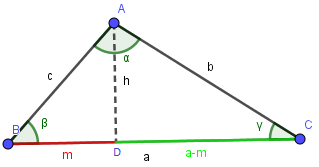
\includegraphics[width=0.50\linewidth]{figures/triangulo.png}
	\end{center}
	\caption{Triângulo para ilustrar a lei dos cossenos.}
	\label{fig:coslaw}
\end{figure}
\begin{itemize}
	\item \textbf{Demonstração Leis dos Cossenos:}
	
	Dado um triângulo qualquer, traça-se uma altura relativa ao lado $a$. Aplicando o \textit{Teorema de Pitágoras} no $\Delta ABD$:
	
	\begin{equation}
	c^{2}=m^{2}+h^{2} \rightarrow h^{2}=c^{2}-m^{2}
	\label{eq:tri1}
	\end{equation}
	
	Aplicando novamente \textit{Pitágoras}, porém, em $\Delta ADC$, obtemos:
	\begin{equation}
	b^{2}=h^{2}+(a-m)^{2}
	\label{eq:tri2}
	\end{equation}
	Substituindo na equação ~\ref{eq:tri2} o valor de $h^{2}$ obtido em ~\ref{eq:tri1}:
	$$
	b^{2}=c^{2}-m^{2}+a^{2}-2am+m^{2}
	$$
	$$
	b^{2}=c^{2}+a^{2}-2am
	$$
	Analisando a 
	Figura ~\ref{fig:coslaw}, pode-se perceber que $\frac{m}{c}=\cos\beta$, então:
	$$
	b^{2}=c^{2}+a^{2}-2ac\cos\beta
	$$
	Analogamente, obtém-se:
	$$
	c^{2}=a^{2}+b^{2}-2ab\cos\gamma
	$$
	$$
	a^{2}=b^{2}+c^{2}-2bc\cos\alpha
	$$
	Note também que se o argumento dos cossenos for $\frac{\pi}{2}$ recaímos no Teorema de Pitágoras. $\hfill\blacksquare$
	\item \textbf{Ângulos Entre 2 Vetores:}
	
	Sejam dois vetores $\overrightarrow{u}$ e $\overrightarrow{v} \in \mathbb{R}^2$, representados na Figura ~\ref{fig:diffbtvet}
	\begin{figure}[H]
		\begin{center}
			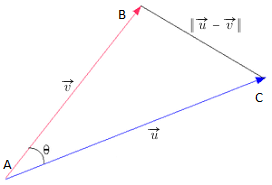
\includegraphics[width=0.4\linewidth]{figures/Angulovetoresnovo.png}
		\end{center}
		\caption{Diferença entre vetores $u$ e $v$}
		\label{fig:diffbtvet}
	\end{figure}
	Para encontrarmos o angulo $\theta$ utilizaremos a lei dos cossenos aplicada a $\Delta ABC$:
	\begin{equation}
	\|\overrightarrow{u}-\overrightarrow{v}\|^{2}=\|\overrightarrow{u}\|^{2} + \|\overrightarrow{v}\|^{2} - 2\|\overrightarrow{u}\|\|\overrightarrow{v}\|\cos\theta
	\label{eq:ang1}
	\end{equation}
	Utilizando a definição do produto escalar \cite{GASteinbruch}
	\begin{equation}
	\|\overrightarrow{u}-\overrightarrow{v}\|^{2}=\|\overrightarrow{u}\|^{2} + \|\overrightarrow{v}\|^{2} - 2\overrightarrow{u}\overrightarrow{v}
	\label{eq:ang2}
	\end{equation}
	Comparando a equação ~\ref{eq:ang1} com a ~\ref{eq:ang2}, obtemos trivialmente
	$$
	\|\overrightarrow{u}\|^{2} + \|\overrightarrow{v}\|^{2} - 2\|\overrightarrow{u}\|\|\overrightarrow{v}\|\cos\theta = \|\overrightarrow{u}\|^{2} + \|\overrightarrow{v}\|^{2} - 2\overrightarrow{u}\overrightarrow{v}
	$$
	$$
	\overrightarrow{u}\overrightarrow{v} = \|\overrightarrow{u}\|\|\overrightarrow{v}\|\cos\theta
	$$
	Logo,
	$$
	\cos\theta = \frac{\overrightarrow{u}\overrightarrow{v}}{\|\overrightarrow{u}\|\|\overrightarrow{v}\|} 
	$$
	$\hfill\blacksquare$
\end{itemize}

\end{document}

